\documentclass[10pt]{article}
\usepackage[utf8]{inputenc}

\title{Granular Dynamic Stochastic Synthesis on the VCV Rack Platform}
\author{
Samuel Laing \\
Advised by Professor Scott Petersen
}
\date{Yale CPSC 490}

\usepackage{natbib}
\usepackage{graphicx}

\usepackage[utf8]{inputenc}
\usepackage[TS1,T1]{fontenc}
\usepackage{fourier, heuristica}
\usepackage{array, booktabs}
\usepackage{graphicx}
\usepackage[x11names,table]{xcolor}
\usepackage{caption}

\usepackage[margin=1.5in]{geometry}
\usepackage{algorithm, algorithmic}

\DeclareCaptionFont{blue}{\color{LightSteelBlue3}}

\newcommand{\foo}{\color{LightSteelBlue3}\makebox[0pt]{\textbullet}\hskip-0.5pt\vrule width 1pt\hspace{\labelsep}}


\begin{document}

\maketitle
\begin{abstract}
The goal of digital sound synthesis processes is often sonic complexity -- to imitate that which is inherent in natural sounds -- while being efficient enough for real-time sound generation. Frequency modulated (FM) synthesis, for instance, accomplishes complexity through the generation of sidebands at frequencies corresponding to the carrier and modulator frequencies. This project focuses on a non-standard, microsound synthesis method, stochastic synthesis, which uses random walks to produce complex, time-varying waves, and presents a novel extension to the synthesis process, as well an implementation as a plugin for the VCV Rack platform. Iannis Xenakis first implemented Dynamic Stochastic Synthesis in 1971 with his GENDY1 program. The synthesis method directly produces and then manipulates a novel waveform using stochastic processes. This project presents an extension to the DSS method through the addition of an underlying synchronous granular synthesis process that informs the interpolation of the stochastic waveform. The granular process granulates sine waves and FM sine waves according to random walks. The resulting form of sound synthesis, Granular Dynamic Stochastic Synthesis (GDSS), maintains much of the sonic character of stochastic synthesis while expanding its sonic range and complexity. Granular Dynamic Stochastic Synthesis is implemented as a generator module for the VCV Rack platform, an open-source modular synthesizer. Two more extensions are presented and implemented as VCV Rack modules: a generator module performing stochastic concatenation of GDSS generated waveforms, and an effects module that uses similar stochastic methods to continually morph a supplied signal. These modules demonstrate the ability of stochastic, microsound synthesis techniques to craft complex waveforms.
\end{abstract}

\pagebreak
\section{Background}
The composer and early computer musician Iannis Xenakis drew heavily upon stochastic processes in the development of his unique musical styles and experiments. Xenakis often used stochastic processes and distributions to map the placement of musical events over time and the frequency spectrum. For instance, in his piece \textit{Pithopraktra}, Xenakis arranges in time and pitch sharp glissandi of 46 string instruments according to Gaussian and Poisson distributions.\citep{xenakis1992} Additionally, in \textit{Analogique A} and \textit{Analogique B} sonic screens with events stochastically distributed throughout are used to shape the tonality and movement of the pieces. 

In each of these pieces, stochastic processes are embedded in the macro controls shaping the density of a cloud, or the sparsity of a section. Xenakis's development of stochastic synthesis moved the stochastic process away from the macro, as it is used to inform a type of microsound synthesis. Microsound synthesis entails the direct manipulation and control of a waveform. Another computer musician pioneering non-standard, microsound synthesis techniques, Herbert Brun, with the technical assistance of Gary Grossman, composed using SAWDUST, a synthesis tool that allowed Brun to "work with the smallest parts of waveforms, to link them and to mingle or merge them with one another."\citep{sergio2006} SAWDUST was, however, a largely deterministic process, and did not embrace the power of stochastic processes like Xenakis's attempt at microsound synthesis.

\subsection{Dynamic Stochastic Synthesis}
 With the help of Marie-Helene Serra, Xenakis implemented Dynamic Stochastic Synthesis (DSS) in his 1971 GENDY1 program written in the BASIC programming language.\citep{xenakis1992} DSS directly synthesizes a wave through the linear interpolation of breakpoints. Breakpoints are an important concept at the core of Xenakis's non-standard micro-sound synthesis method. Each breakpoint represents a point, an amplitude, and a duration value, in the wave being produced. After each cycle, each breakpoint takes a step where its amplitude and duration values are altered by a random walk. As a result, the wave being produced will continually morph and step its way through sonic space, bringing in and taking out numerous complicated transients in the process. It is the small, incremental walks of each breakpoint that give stochastic synthesis its unique and complex sonic character.

\subsection{Existing Implementations and Extensions}
Since Xenakis first introduced DSS there have been several attempts to extend the method of synthesis and to bring it to new platforms. Nick Collins adapted Xenakis's DSS to the SuperCollider3 platform with his Gendy1, Gendy2, and Gendy3 UGens, and even implemented a Gendy synthesis engine for the iPhone.\citep{collins2011} These implementations focus on the stochastic richness of stochastic synthesis, implementing first-order and then second-order random walks. Additionally, they expose stochastic synthesis to a greater user base on the SuperCollider3 platform. Luc Dobereiner's PHINGEN, or Physically Informed Stochastic Synthesis, is another novel extension to DSS synthesis that replaces the linear interpolation between breakpoints with a physical model.\citep{luc2011dobereiner} PHINGEN is also available on the SuperCollider3 platform as a UGen.

\section{Extending Dynamic Stochastic Synthesis}
To extend Xenakis's stochastic synthesis, I incorporated another synthesis type: granular synthesis. DSS generally utilizes linear interpolation to calculate samples in-between breakpoints. If a small number of breakpoints is used, the complexity of produced sounds can be limited. By incorporating a synchronous granular synthesis method into the interpolation process, I have introduced the ability to add micro-variations to the DSS wave. 

The incorporation of granular synthesis into stochastic synthesis begins with the expansion of the breakpoint. For stochastic synthesis, the breakpoint represents only amplitude and duration values. Grain offset and grain rate values are added to each breakpoint in order to inform the granular synthesis. Granular synthesis requires a sonic resource or raw material that is to be enveloped. To avoid the added complexity of sample storage, or input signal granulation, GDSS uses sine waves, or single-carrier single-modulator FM sine waves, as the sonic material. Algorithm 1 shows pseudocode for the process that computes each amplitude of the stochastic wave. Within the \texttt{if} statement, breakpoint stepping occurs. Below the if statement is the granular interpolation step that is responsible for \textit{joining} breakpoints.

\begin{algorithm}\captionsetup{labelfont={sc,bf}, labelsep=newline}
\caption{Granular Dynamic Stochastic Synthesis Algorithm}
    \begin{algorithmic}
        \STATE $breakpoints\gets [\{amp,\ dur,\ off,\ grate\}]$
        \STATE $i\gets 0$
        \STATE $prob\_dist\gets UNIFORM$
        \STATE $phase\gets1.0$
        \LOOP
            \IF{$phase >= 1.0$}
                \STATE $i++$
                \STATE $breakpoints_{i}.amp += rand(prob\_dist)$
                \STATE $breakpoints_{i}.dur += rand(prob\_dist)$
                \STATE $breakpoints_{i}.off += rand(prob\_dist)$
                \STATE $breakpoints_{i}.grate += rand(prob\_dist)$
            \ENDIF
            \STATE $amp\gets breakpoints_{i-1}.amp + (env * sinf(breakpoints_{i-1}.off))$
            \STATE $amp\_next\gets breakpoints_{i}.amp + (env\_next * sinf(breakpoints_{i}.off))$
            \STATE $amp\_out\gets ((1.0 - phase) * amp) + (phase * amp\_next)$
            \STATE $speed\gets freq * breakpoints_{i}.dur * bpts.size$
            \STATE $phase += speed$
            \STATE $sample\_out(amp\_out)$
        \ENDLOOP
    \end{algorithmic}
\end{algorithm}


\subsection{The Stochastic Method as Effect}
DSS and now GDSS are both generative processes using random walks to continually alter the produced sound. The same stochastic process can, instead, be used as a means for sonic effect through application to an existing waveform. I present a method of morphing a sampled waveform using the random walks of breakpoints. Each breakpoint still represents an amplitude and duration value, but now the breakpoints correspond to the length and amplitude of an envelope, which is to be applied to a section of the sample wave. Algorithm 2 shows how the breakpoints are applied through amplitudes to the store sample. The envelopes distribute the breakpoint's amplitude to nearby samples, and the incremental changes they apply to the stored waveform lead to the generation of a wave different than what was input.

\begin{algorithm}\captionsetup{labelfont={sc,bf}, labelsep=newline}
\caption{Stochastic Effect Algorithm}
    \begin{algorithmic}
        \STATE $breakpoints\gets [\{amp,\ dur\}]$
        \STATE $i\gets 0$
        \STATE $prob\_dist\gets UNIFORM$
        \STATE $sample\gets [float]$
        \STATE $env\gets TRI$
        \LOOP
            \IF{$phase >= 1.0$}
                \STATE $index++$
                \STATE $breakpoints_{i}.amp += rand(prob\_dist)$
                \STATE $breakpoints_{i}.dur += rand(prob\_dist)$
            \ENDIF
            \STATE $amp\_out\gets sample[i] + (env[g_i] * breakpoints_{i}.amp)$
            \STATE $sample[i]\gets amp\_out$
            \STATE $speed\gets freq * breakpoints_{i}.dur * breakpoints.size$
            \STATE $phase += speed$
            \STATE $sample\_out(amp\_out)$
        \ENDLOOP
    \end{algorithmic}
\end{algorithm}

\subsection{Goals}
The goals of this project are as follows: To alter the method of stochastic synthesis to extend its tonal and timbral range through the addition of granular processes. To expand on the implementation offerings for stochastic and microsound synthesis techniques. To offer the resulting synthesis type in a form that facilitates musical and experimental use.

\section{Implementation and Modules}
There are many existing platforms and technologies for the development of DSP plugins: Will Perkle's RackAFX, SuperCollider3, VST, Audio Units, and so on.\citep{rackafx} I chose to use a new platform, VCV Rack, which simulates modular synthesizer hardware. VCV Rack is a fully open-source program that was started in 2016 by Andrew Belt, and has recently gained popularity in the world of music-software technology.\citep{vcvrack} Unlike the SuperCollider3 UGen interface, samples in VCV Rack are not generated in blocks, rather each sample is generated individually. While this method of sample generation is less efficient and less easily parallelized, it adheres more closely to the modular synth paradigm.

\subsection{VCV Rack Plugin Development}

VCV Rack facilitates the development of new modules, or plugins, for the platform by exposing the \texttt{Model} class, which accepts \texttt{Module} and \texttt{ModuleWidget} structs. The \texttt{Module} struct is responsible for the plugin's logic. The Rack engine calls \texttt{Module.step()} during each cycle. Each sample output by the module is calculated and output within the \texttt{step} function. The \texttt{ModuleWidget} handles the UI for the module and specifies the type and location of controls for the panel. Each of the modules described below was implemented by extending the \texttt{Module} and \texttt{ModuleWidget} \texttt{structs} to create a new \texttt{Model}. All together, the modules are released as a package to the VCV Rack community under the name \texttt{StochKit}, short for Stochastic Toolkit.

\subsection{GRANDY}
The main module of the stochastic suite is the GRANDY module. GRANDY is a generator module that implements Granular Dynamic Stochastic Synthesis. The module is modeled after other voltage controlled oscillator (VCO) modules since it is to serve a similar purpose in a modular synthesizer user's toolkit. Most parameters for controlling Granular Dynamic Stochastic Synthesis, such as frequency, the number of breakpoints, the maximum step in amplitude values, the maximum step in duration values, probability distribution, grain frequency, and so on, are exposed through the panel's knobs. Other parameters, such as maximum grain offset step and maximum grain rate, are not available for control, as experiments discerned that these variables do not return \textit{predictable} changes when modulated. Instead, the granular synthesis is more intuitively controlled through altering the sonic material that is being granulated. This is possible through grain frequency and envelope window type controls.

\begin{figure}
  \caption{The VCV Rack Grandy module.}
  \centering
    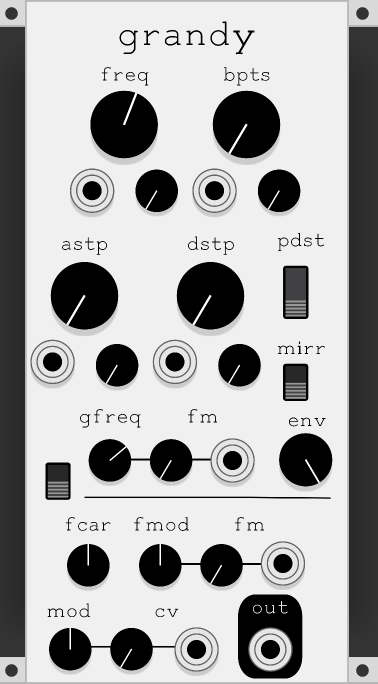
\includegraphics[height=0.25\textheight]{grandy}
\end{figure}

\subsection{STITCHER}
Sergio Luque, in the paper \textit{Stochastic Synthesis: Origins and Extensions}, presents the method of stochastic concatenation as an extension of Xenakis's original stochastic synthesis.\citep{sergio2006} The process does not alter the core method of stochastic synthesis but presents a method of stochastic orchestration of several stochastic synthesizers where multiple stochastic synthesis generators produce waves that are concatenated one after another to form a new output wave. 

The STITCHER module, shown in Figure 2, implements stochastic concatenation, as described by Luque, using GRANDY instead of GENDYN generators. Each oscillator can be controlled separately, or by a set of global parameter knobs. The wave output by the module is a successive concatenation of waves output by each of the GRANDY oscillators.

Luque describes the concatenation of stochastic waves as being influenced by tendency masks, or other stochastic processes.\citep{sergio2006} In order to translate the selection method into a VCV Rack module, my implementation, instead, allows the user or musician control over this process. The number of wave cycles a single oscillator outputs before the next oscillator is used, and whether an oscillator is active in the synthesis at a given time, are both parameters the user may control using the corresponding knobs. While a significant stochastic element is removed, the musical uses of the technique are expanded by giving the user greater control over the synthesis.

\begin{figure}
  \caption{The VCV Rack Stitcher module.}
  \centering
    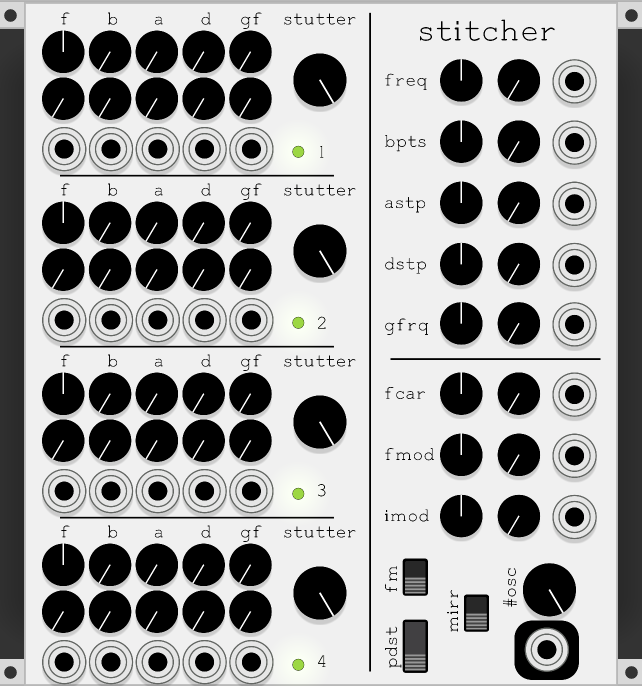
\includegraphics[height=0.25\textheight]{stitcher}
\end{figure}

\subsection{GenECHO}
Unlike the GRANDY and STITCHER modules, the GenECHO module, shown in Figure 3, is not a generator, but an effects module. On a gate input, the module samples an input signal and proceeds to apply a \textit{stochastic decomposition} to the sampled wave. GenECHO, like GRANDY, maintains a number of breakpoints, but each breakpoint only contains an amplitude and duration value. The number of breakpoints is influenced by the length of the sample being \textit{echoed} and a controllable breakpoint-spacing parameter. As the wave is repeatedly looped through, each breakpoint applies an envelope with a stochastically-generated amplitude to the stored sample, as described by Algorithm 2. Over time, the stored sample is increasingly morphed by the stochastic shifts, causing new sounds to appear and the original sound to become \textit{lost}.

\begin{figure}
  \caption{The VCV Rack GenEcho module.}
  \centering
    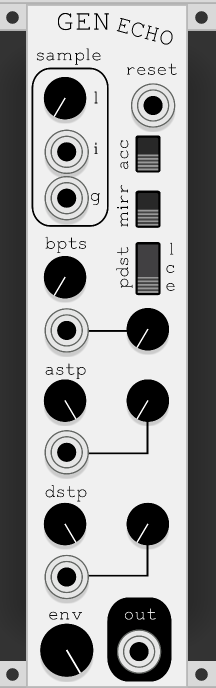
\includegraphics[height=0.25\textheight]{genecho}
\end{figure}

\section{Results}
The completed modules are available for download and use with the VCV Rack Platform through the VCV Plugin Manager. The GRANDY oscillator demonstrates Granular Dynamic Stochastic Synthesis's ability to produce a wide range of complex sounds, both those that sound similar to those generated by GENDYN and beyond. The STITCHER module, especially, produces a large variety of sounds even with only four GRANDY oscillators being used. The adaptation of stochastic synthesis methods to the VCV Rack platform was successful and opens up a wide range of sonic and aesthetic possibilities to those using the VCV Rack platform. Due to VCV Rack's open nature, and deeply integrated plugin management system, these plugins are available to download and use by all VCV Rack users at the click of a button.

\section{Acknowledgements}
There is no end to the number of people I would like to thank. First, my advisor, Scott Peterson, for his invaluable help with this project and much-needed humor. My sister, Sophie, for her never-ending support. My parents, Kate and Charlie, for their interest in my work. And, of course, my friends, Gabe and Rachel to name a few, for tolerating all the strange sounds that this project has produced.

\pagebreak
\bibliographystyle{plain}
\bibliography{references}

\end{document}
